\documentclass[12pt, a4paper]{article}

\usepackage[hmargin=2.5cm, vmargin=2cm]{geometry}
\usepackage{amsthm, amssymb, mathtools, yhmath, graphicx}
\usepackage{fontspec, type1cm, titlesec, titling, fancyhdr, tabularx}
\usepackage{color}
\usepackage{unicode-math}
\usepackage{float}
\usepackage{subfig}
\usepackage{hhline}
\usepackage{comment}
\usepackage{siunitx}
\usepackage{csvsimple}
\usepackage{subcaption}

\usepackage[CheckSingle, CJKmath]{xeCJK}
\usepackage{CJKulem}
\usepackage{enumitem}
\usepackage{tikz}
\usepackage[siunitx]{circuitikz}
\usepackage{wrapfig}
%\setCJKmainfont[BoldFont=cwTex Q Hei]{cwTex Q Ming}
%\setCJKsansfont[BoldFont=cwTex Q Hei]{cwTex Q Ming}
%\setCJKmonofont[BoldFont=cwTex Q Hei]{cwTex Q Ming}
%\setCJKmainfont[BoldFont=cwTeX Q Hei]{cwTeX Q Ming}
\setmainfont{Linux Libertine O}
\setCJKmainfont[BoldFont=cwTeX Q Hei]{cwTeX Q Ming}

\def\normalsize{\fontsize{12}{18}\selectfont}
\def\large{\fontsize{14}{21}\selectfont}
\def\Large{\fontsize{16}{24}\selectfont}
\def\LARGE{\fontsize{18}{27}\selectfont}
\def\huge{\fontsize{20}{30}\selectfont}

%\titleformat{\section}{\bf\Large}{\arabic{section}}{24pt}{}
%\titleformat{\subsection}{\large}{\arabic{subsection}.}{12pt}{}
%\titlespacing*{\subsection}{0pt}{0pt}{1.5ex}

\parindent=24pt

\DeclarePairedDelimiter{\abs}{\lvert}{\rvert}
\DeclarePairedDelimiter{\norm}{\lVert}{\rVert}
\DeclarePairedDelimiter{\inpd}{\langle}{\rangle}
\DeclarePairedDelimiter{\ceil}{\lceil}{\rceil}
\DeclarePairedDelimiter{\floor}{\lfloor}{\rfloor}

\newcommand{\unit}[1]{\:(\text{#1})}
\newcommand{\df}[1]{\mathop{}\!\mathrm{d^#1}}
\newcommand{\img}{\mathrm{i}}
\newcommand{\dD}{\mathrm{d}}
\newcommand{\dI}{\,\mathrm{d}}

\title{ \bf {\Huge 電子電路實驗4: Multiple Feedback Network  }\\ 實驗結報}
\author{B02901178 江誠敏}

\begin{document}

\maketitle


\section{實驗結果}
\begin{center}
\begin{tabular}{p{3cm}p{3cm}}
	\hline
  Item & Value\\
	\hhline{==}
  $f_o$ & $\SI{344}\Hz$ \\
  $V_{o(p-p)}$ & $\SI{5.361}\V$ \\
  $V_{s(p-p)}$ & $\SI{52.8}\mV$ \\
  $V_{j(p-p)}$ & $\SI{1.30}\V$ \\
  $R_{p1}$ & $\SI{2.6}\kohm$ \\
  $R_{p2}$ & $\SI{7.9}\kohm$ \\
	\hline
\end{tabular}
\end{center}
\section{結報問題}

\begin{enumerate}[itemsep=20pt, topsep=10pt]

  \item {請描述基本迴授電路 4 大組態。} \\[10pt]
    答:
    \begin{itemize}
      \item Series-shunt
        \begin{figure}[H]
          \centering
          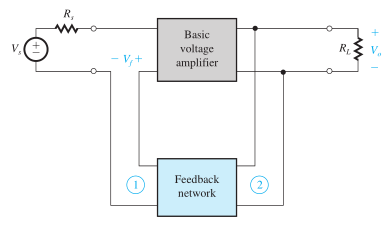
\includegraphics[width=0.5\textwidth]{img/sesh.png}
        \end{figure}
        Feedback network 的輸入端與原電路並聯,也就是輸入端接收電壓。\\
        輸出端則與原電路串聯,也就是輸出端輸出電壓。

      \item Shunt-series
        \begin{figure}[H]
          \centering
          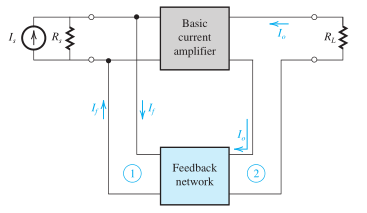
\includegraphics[width=0.5\textwidth]{img/shse.png}
        \end{figure}
        Feedback network 的輸入端與原電路串聯,也就是輸入端接收電流。\\
        輸出端則與原電路並聯,也就是輸出端輸出電流。

      \item Series-series
        \begin{figure}[H]
          \centering
          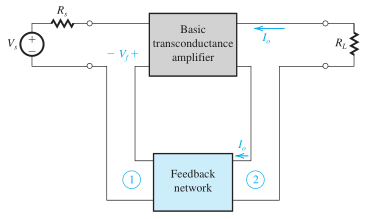
\includegraphics[width=0.5\textwidth]{img/sese.png}
        \end{figure}
        Feedback network 的輸入端與原電路串聯,也就是輸入端接收電流。\\
        輸出端則與原電路串聯,也就是輸出端輸出電壓。

      \item Shunt-shunt
        \begin{figure}[H]
          \centering
          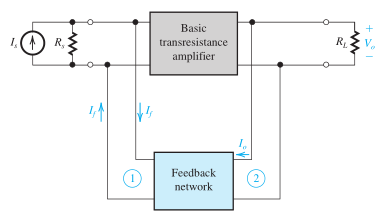
\includegraphics[width=0.5\textwidth]{img/shsh.png}
        \end{figure}
        Feedback network 的輸入端與原電路並聯,也就是輸入端接收電壓。\\
        輸出端則與原電路並聯,也就是輸出端輸出電流。

    \end{itemize}
      

  \item {請詳述如何準確判別迴授電路的形態。} \\[10pt]
    答:\\
    首先把電路的放大電路還有迴授電路分離出來,接著辨斷迴授電路的輸入、
    輸出端分別是用哪一種方法被連接到放大電路上,如此由上一題的結果就
    可以準確判斷迴授電路的形態。

\end{enumerate}

\section{心得}
這次的實驗其實還蠻酷的,用一個 \SI{10}\Hz 的方波居然可以製造出一個
頻率高很多的弦波,而且這次的實驗步驟又很短,也沒有什麼比較容易出錯的
地方,電路也不會說太複雜,可以說是簡單又有趣!
\end{document}

